\documentclass{ctexart}
\usepackage[T1]{fontenc}
\usepackage[a4paper,top=1.5cm,bottom=1.5cm,left=2cm,right=2cm,marginparwidth=1.75cm]{geometry}
\usepackage{mathtools}
\usepackage{tikz}
\usepackage{flexisym}
\usepackage{breqn}
\usepackage{booktabs}
\usepackage{caption}
\usepackage{outlines}
\usepackage{graphicx}
\usepackage{float}
\usepackage{amsthm}
\usepackage{tabularray}
\usepackage{minted}
\usepackage[colorlinks=false, allcolors=blue]{hyperref}
\usepackage{cleveref}
\renewcommand{\tableautorefname}{表}
\DeclarePairedDelimiter{\set}{\{}{\}}
\DeclarePairedDelimiter{\paren}{(}{) }
\graphicspath{ {./images/} }

\newcounter{fullrefcounter}
\newcommand*{\fullref}[1]{%
\addtocounter{fullrefcounter}{1}%
\label{--ref-\thefullrefcounter}%
\ifthenelse{\equal{\getpagerefnumber{--ref-\thefullrefcounter}}{\getpagerefnumber{#1}}}
  {
    \hyperref[{#1}]{\Cref*{#1} \nameref*{#1}}
  }
  {% false case
    \hyperref[{#1}]{第 \pageref*{#1} 页 \Cref*{#1} \nameref*{#1}}
  }
}

\title{编译原理第二次作业}
\author{卢雨轩 19071125}
% \date{\today}
\ctexset{
    section = {
        titleformat = \raggedright,
        name = {,},
        number = \chinese{section}、
    },
    paragraph = {
        runin = false
    },
    today = small,
    figurename = 图,
    contentsname = 目录,
    tablename = 表,
}

\begin{document}

\maketitle

\begin{outline}
    \1 [23.]
        \2[(8)] $0(0|1) ^*1$
    \1 [27.]
        \2[(1)] \begin{dmath*}
            (1|2|3|4|5|6|7|8|9) (0|1|2|3|4|5|6|7|8|9) ^3.((1|3|5|7|8|10|12) .((\epsilon|1|2) (0|1|2|3|4|5|6|7|8|9) |30|31) ) |((4|6|9|11) . \\ 
            ((\epsilon|1|2) (0|1|2|3|4|5|6|7|8|9) |30) |2.(\epsilon|1|2) (0|1|2|3|4|5|6|7|8|9) ) 
        \end{dmath*}
        \2[(2)] \begin{dmath*}
            (
            (
                ((\epsilon|1|2) (0|1|2|3|4|5|6|7|8|9) |30|31)\; (1|3|5|7|8|10|12)
            ) |
            ((\epsilon|1|2) (0|1|2|3|4|5|6|7|8|9) |30)\;(4|6|9|11) | \\(\epsilon|1|2) (0|1|2|3|4|5|6|7|8|9)\;2
            )\;(1|2|3|4|5|6|7|8|9) (0|1|2|3|4|5|6|7|8|9) ^3
        \end{dmath*}
        \2[(3)] \begin{dmath*}
            ((1|3|5|7|8|10|12)/((\epsilon|1|2) (0|1|2|3|4|5|6|7|8|9) |30|31) ) |((4|6|9|11) /\\ 
            ((\epsilon|1|2) (0|1|2|3|4|5|6|7|8|9) |30) |2/(\epsilon|1|2) (0|1|2|3|4|5|6|7|8|9) )/(1|2|3|4|5|6|7|8|9) (0|1|2|3|4|5|6|7|8|9) ^3
        \end{dmath*}
    \1 [31] \2[(2)]
\end{outline}


\begin{figure}[H]
    \centering
    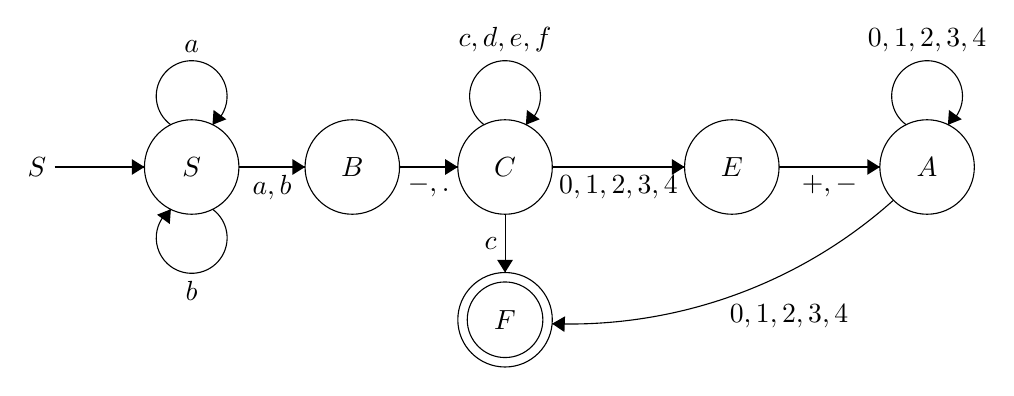
\begin{tikzpicture}[scale=0.2]
    \tikzstyle{every node}+=[inner sep=0pt]
    \draw [black] (17.8,-13.2) circle (3);
    \draw (17.8,-13.2) node {$S$};
    \draw [black] (28,-13.2) circle (3);
    \draw (28,-13.2) node {$B$};
    \draw [black] (37.7,-13.2) circle (3);
    \draw (37.7,-13.2) node {$C$};
    \draw [black] (37.7,-22.9) circle (3);
    \draw (37.7,-22.9) node {$F$};
    \draw [black] (37.7,-22.9) circle (2.4);
    \draw [black] (52.1,-13.2) circle (3);
    \draw (52.1,-13.2) node {$E$};
    \draw [black] (64.5,-13.2) circle (3);
    \draw (64.5,-13.2) node {$A$};
    \draw [black] (9.1,-13.2) -- (14.8,-13.2);
    \draw (8.6,-13.2) node [left] {$S$};
    \fill [black] (14.8,-13.2) -- (14,-12.7) -- (14,-13.7);
    \draw [black] (16.477,-10.52) arc (234:-54:2.25);
    \draw (17.8,-5.95) node [above] {$a$};
    \fill [black] (19.12,-10.52) -- (20,-10.17) -- (19.19,-9.58);
    \draw [black] (19.123,-15.88) arc (54:-234:2.25);
    \draw (17.8,-20.45) node [below] {$b$};
    \fill [black] (16.48,-15.88) -- (15.6,-16.23) -- (16.41,-16.82);
    \draw [black] (20.8,-13.2) -- (25,-13.2);
    \fill [black] (25,-13.2) -- (24.2,-12.7) -- (24.2,-13.7);
    \draw (22.9,-13.7) node [below] {$a,b$};
    \draw [black] (31,-13.2) -- (34.7,-13.2);
    \fill [black] (34.7,-13.2) -- (33.9,-12.7) -- (33.9,-13.7);
    \draw (32.85,-13.7) node [below] {$-,.$};
    \draw [black] (36.377,-10.52) arc (234:-54:2.25);
    \draw (37.7,-5.95) node [above] {$c,d,e,f$};
    \fill [black] (39.02,-10.52) -- (39.9,-10.17) -- (39.09,-9.58);
    \draw [black] (37.7,-16.2) -- (37.7,-19.9);
    \fill [black] (37.7,-19.9) -- (38.2,-19.1) -- (37.2,-19.1);
    \draw (37.2,-18.05) node [left] {$c$};
    \draw [black] (40.7,-13.2) -- (49.1,-13.2);
    \fill [black] (49.1,-13.2) -- (48.3,-12.7) -- (48.3,-13.7);
    \draw (44.9,-13.7) node [below] {$0,1,2,3,4$};
    \draw [black] (55.1,-13.2) -- (61.5,-13.2);
    \fill [black] (61.5,-13.2) -- (60.7,-12.7) -- (60.7,-13.7);
    \draw (58.3,-13.7) node [below] {$+,-$};
    \draw [black] (63.177,-10.52) arc (234:-54:2.25);
    \draw (64.5,-5.95) node [above] {$0,1,2,3,4$};
    \fill [black] (65.82,-10.52) -- (66.7,-10.17) -- (65.89,-9.58);
    \draw [black] (62.366,-15.306) arc (-48.16435:-92.04119:30.852);
    \fill [black] (40.69,-23.15) -- (41.47,-23.68) -- (41.51,-22.68);
    \draw (55.73,-21.93) node [below] {$0,1,2,3,4$};
    \end{tikzpicture}
    \end{figure}
\end{document}
